\chapter{Kravspesifikasjon}
\label{chap:kravspesifikasjon}
Dette kapitlet inneholder funksjonelle og operasjonelle krav som gjelder for autentisering- og autoriseringløsningen Norkart trenger. Det vil være beskrevet og presentert noen use caser i \ref{subsec:kravspesifikasjon_funksjonelleKrav_hoyNivaa} \nameref{subsec:kravspesifikasjon_funksjonelleKrav_hoyNivaa}.

\section{Hvordan kravspesifikasjon er utarbeidet}
\label{sec:kravspesifikasjon_hvordanKravspesifikasjonErUtarbeidet}
Prosjektgruppen brukte et par uker på å sette seg inn i ulike autentiseringsløsninger før kravspesifikasjonen ble utarbeidet. Gruppen utarbeidet kravspesifikasjonen tidlig i prosessen i samråd med product owner hos Norkart. Denne ble oppdatert etterhvert som det skjedde endringer i prosjektet slik at den samsvarte med oppgaven til en hver tid. Etter at valget av autentiseringsverktøy ble tatt ble kravspesifikasjonen oppdatert til å inneholdet krav for mer enn det oppgaven først tilsa. I forhold til målbare data oppgitt i seksjon \ref{sec:kravspesifikasjon_operasjonelleKrav} -  \nameref{sec:kravspesifikasjon_operasjonelleKrav} tok vi utgangspunkt i hva Norkart så for seg som et ekstremscenario for løsningen om de skulle selge svært mye og ha mye aktivitet. 
 
\section{Funksjonelle krav til løsningen}
\label{sec:kravspesifikasjon_funksjonelleKrav}
Oppgavens funksjonelle krav har til hensikt å forklare hva slags funksjonalitet løsningen skal tilby og hvilke roller som har tilgang til de forskjellige funksjonene. Disse kravene skal også vise hvordan systemet skal reagere på ulike situasjoner.

\subsection{Overordnet use case diagram}
\label{subsec:kravspesifikasjon_funksjonelleKrav_OverordnetUseCase}
For å beskrive hva Norkart ønsker i løsningen er det laget et overordnet use case  (se figur \ref{fig:OverordnetUseCase}). Use caset viser hovedfunksjonene til løsningen, samt hvilke roller som skal bruke hvilke funksjonalitet. Nedenfor vil du kunne lese en kort forklaring av roller og funksjoner.

\begin{figure}[h]
    \begin{center}
        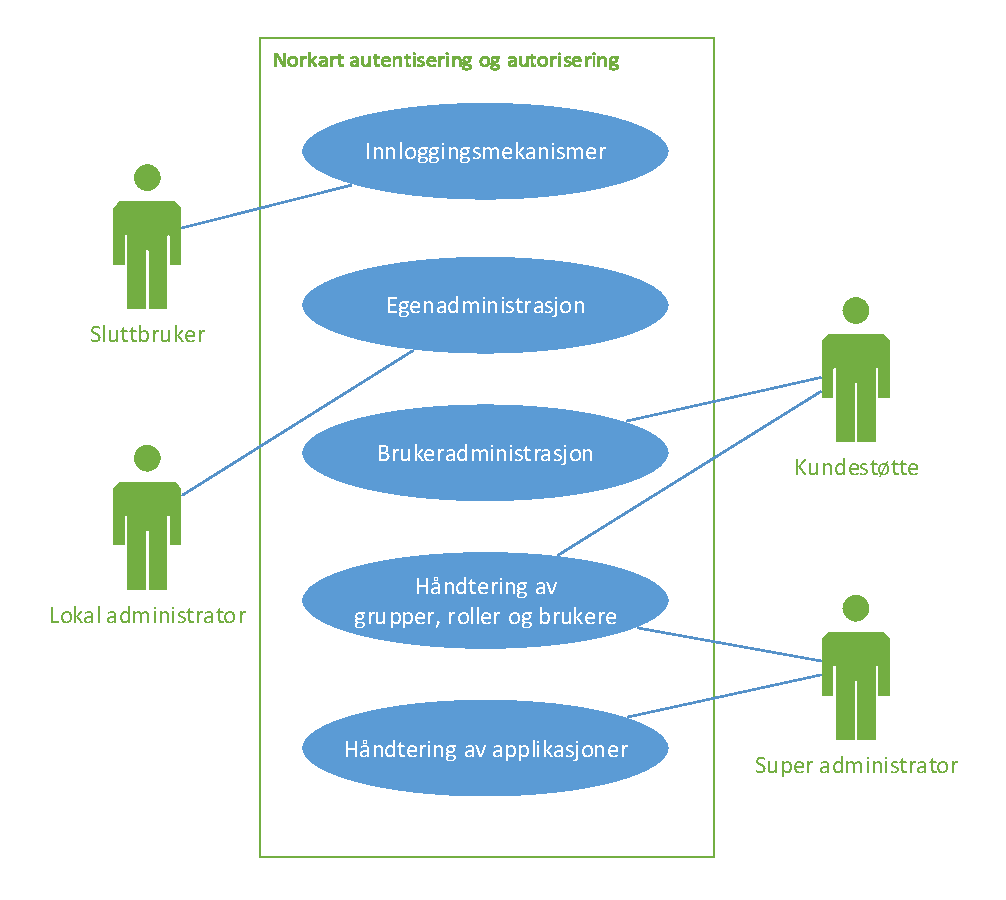
\includegraphics[scale=0.65]{graphics/OverordnetUseCase}
        \caption{overordnet Use Case for autentisering- og autoriseringløsning til Norkart}
        \label{fig:OverordnetUseCase}
        \end{center}
\end{figure}

\subsubsection*{Super administrator}
Super administrator er rollen som administrerer og konfigurerer AAD. Denne rollen er hovedsakelig ment for utviklere og driftere i Norkart. De vil ha mulighet til å håndtere applikasjoner som skal bruke løsningen i tillegg til å håndtere grupper og roller i AAD. 

\subsubsection*{Kundestøtte}
Kundestøtte rollen vil si de som jobber hos kundestøtte i Norkart. De kan hjelpe brukere med funksjonalitet innen brukeradministrasjon. De kan også håndtere grupper og roller i AAD.

\subsubsection*{Lokal administrator}
Denne rollen har til hensikt å administrere brukere innenfor en gitt gruppe. Det kan enten være en person som jobber hos Norkart eller en lokal administrator innenfor en bedrift som benytter seg av NorkartID. Rollen resulterer i redusert press på Norkart kundestøtte.

\subsubsection*{Sluttbruker}
Sluttbruker bruker løsningen som autentisering og autoriseringtjeneste. Dette er brukerne som logger inn via løsningen og får tilgang til tjenestene Norkart tilbyr. I tillegg til dette har de også tilgang på egenadministrasjon slik at belastningen på kundestøtte hos Norkart reduseres ytterligere.

\subsection{Høynivå use case beskrivelser}
\label{subsec:kravspesifikasjon_funksjonelleKrav_hoyNivaa}
For å skape forståelse rundt hovedfunksjonalitet i løsningen er det utviklet 5 høynivå use case beskrivelser.

\begin{framed}
    \begin{tabular}{l p{9cm}}
        \textbf{Use case:} & Innloggingsmekanismer \\
        \textbf{Aktører:} & Sluttbruker
        \bigskip \\
        \textbf{Mål:} & Aktør skal kunne logge seg inn og få sikker tilgang til ønsket applikasjon. Dette skal være SSO slik at aktør i tillegg blir autentisert for andre applikasjoner aktør har tilgang til. Aktør skal i tillegg kunne logge seg ut av en applikasjon. Det skal også være mulig for aktør å gjenopprette sitt eget passord dersom dette er glemt.
        \bigskip \\
        \textbf{Beskrivelse:} & For å skape oversikt deles innloggingsmekanismer her opp i tre underkategorier, logg inn, logg ut og glemt passord. 
        \bigskip \\ 
        \textit{Logg inn} & Når aktør skriver inn brukernavn og passord skal aktøren autentiseres og få tilgang til applikasjonen det ønskes å jobbe på. Da skal aktøren også bli autentisert for andre applikasjoner uten å måtte oppgi brukernavn og passord på nytt. Det vil altså si at det skal være en SSO løsning. 
        \bigskip \\
        \textit{Logg ut} & Når aktør klikker logg ut skal brukeren bli utlogget fra applikasjonen.
        \bigskip \\
        \textit{Glemt passord} & Hvis aktør glemmer sitt passord skal det være mulig å gjenopprette sitt eget passord uten å måtte kontakte Norkart kundestøtte. Aktøren skal kunne gjøre dette ved å trykke på en glemt passord lenke på innloggingsiden. Det skal da sendes en verifiseringkode enten via e-post eller telefon. Ved å oppgi denne koden skal aktøren selv kunne opprette et nytt passord.
    \end{tabular}
\end{framed}

\begin{framed}
    \begin{tabular}{l p{9cm}}
        \textbf{Use case:} & Egenadministrasjon \\
        \textbf{Aktører:} & Sluttbruker 
        \bigskip \\
        \textbf{Mål:} & Aktør skal selv kunne endre {\color{red}og registrere?} på egne registrerte opplysninger på sin brukerprofil. 
        \bigskip \\
        \textbf{Beskrivelse:} &  Aktør skal selv kunne endre sitt registrerte mobilnummer, ekstern e-post adresse og sitt passord. For å endre passord må aktør først oppgi sitt gamle passord, for deretter å skrive inn det nye passordet to ganger. Aktør får kun tilgang til å endre egne data etter å ha blitt autentisert. Egenadministrasjon skal foregå i en ekstern brukerportal, altså ikke i Azure portalen.
    \end{tabular}
\end{framed}

\begin{framed}
    \begin{tabular}{l p{9cm}}
        \textbf{Use case:} & Brukeradministrasjon \\
        \textbf{Aktører:} & Lokal administrator og kundestøtte 
        \bigskip \\
        \textbf{Mål:} & Håndtere brukere innenfor en gitt gruppe.  
        \bigskip \\
        \textbf{Beskrivelse:} & Aktør skal kunne registrere brukere og legge disse til i grupper aktør har tilgang til. Aktør skal i tillegg kunne resette passord for brukerne som er registrert i disse gruppene. Dette skal kunne gjøres fra en egen nettside.
    \end{tabular}
\end{framed}

\begin{framed}
    \begin{tabular}{l p{9cm}}
        \textbf{Use case:} & Håndtering av grupper, roller og brukere \\
        \textbf{Aktører:} & Kundestøtte og super administrator 
        \bigskip \\
        \textbf{Mål:} & Aktør skal kunne registrere og håndtere brukere, grupper og roller.
        \bigskip \\
        \textbf{Beskrivelse:} & For å skape oversikt beskrives brukere, grupper og roller hver for seg.
        \bigskip \\
        \textit{Brukere} & Aktør skal kunne registrere enkeltbrukere i AAD. I tillegg skal det være mulig å masseregistrere brukere fra en ekstern kilde. Aktør skal også kunne legge brukere til i grupper, tildele roller til brukerne og administrere brukernes tilgang til applikasjoner. Dette skal kunne gjøres i Azure portalen.
        \bigskip \\
        \textit{Grupper} & Aktør skal kunne opprette grupper og administrere disse i Azure portalen slik at Norkart kan ha plassere brukere i grupper med forskjellige rettigheter og tilganger. 
        \bigskip \\
        \textit{Roller} & Aktør skal kunne opprette roller med forskjellige rettigheter og tildele disse til brukere som er registrert i AAD. I tillegg skal aktør kunne konfigurere rettigheter og tilganger for eksisterende roller.
    \end{tabular}
\end{framed}

\begin{framed}
    \begin{tabular}{l p{9cm}}
        \textbf{Use case:} & Håndtering av applikasjoner \\
        \textbf{Aktører:} & Super administrator
        \bigskip \\
        \textbf{Mål:} & Aktør skal kunne registrere og administrere applikasjoner i en AAD. I tillegg skal aktør kunne klargjøre applikasjoner for bruk av løsningen.
        \bigskip \\
        \textbf{Beskrivelse:} & I Azure portalen skal aktør kunne registrere web applikasjoner og native applikasjoner for bruk av autentiseringløsningen. Aktør skal også kunne administrere applikasjonenes tilganger og annen informasjon her. I tillegg skal aktør kunne klargjøre og implementere nødvendig logikk i applikasjonene som skal bruke løsningen.
    \end{tabular}
\end{framed}

\section{Operasjonelle krav til løsning}
\label{sec:kravspesifikasjon_operasjonelleKrav}
Operasjonelle krav brukes for å beskrive kvaliteten på systemet og dette kan være i form av standarder som benyttes eller målinger innenfor en gitt grense og kostnader.

\subsection{Ytelse}
\label{subsec:kravspesifikasjon_operasjonelleKrav_ytelse}
\begin{itemize}
\item Løsningen skal som minimum takle 10 000 brukere innlogget samtidig.
\item Løsningen skal håndtere pålogging av 100 brukere i minuttet.
\item Løsningen skal bygges for å være skalerbar.
\item Verifiseringskode for resetting av passord skal mottas innen 20 sekunder for både e-post og telefon.
\end{itemize}

\subsection{Brukervennlighet}
\label{subsec:kravspesifikasjon_operasjonelleKrav_brukervennlighet}
\begin{itemize}
\item Løsningen skal følge regler for universell utforming, se Lover og regler \ref{subsec:kravspesifikasjon_operasjonelleKrav_loverOgRegler}
\item Bruker skal kunne bruke samme pålogginginformasjon mot alle systemene til Norkart.
\item Innloggingsmekanismer som å logge innog egenadministrasjon, se høynivå use case beskrivelse \ref{subsec:kravspesifikasjon_funksjonelleKrav_hoyNivaa}, skal kunne utføres uten opplæring.
\item Brukergrensesnittet, heretter GUI, på innloggingssiden skal være så intuitivt at det tar mindre enn 2 sekunder å skjønne hvor brukerid felt, passord felt og innloggingknappen er.
\item Etter at innloggingsknappen er trykt skal det ta mindre enn 2 sekunder før brukeren ser at noe skjer.
\item Logg ut knappen skal være synlig for bruker i hele applikasjonen
\item Brukeren skal få respons på at utlogging er utført.
\item Når bruker lager passord skal det gis indikasjon på om passordkravene tilfredstilles
\item Brukerprofil for egenadministrasjon skal være oversiktlig og brukeren skal selv skjønne hva som skal gjøres for å endre brukerdata.
\item GUI for all konfigurering av AAD skal være oversiktlig nok til at bruker kan utføre use casene håndtering av brukere, grupper og roller og håndtering av applikasjoner etter å ha fått innføring i Azure eller lest rapporten.
\item GUI design skal skape gjenkjennelighet til Norkart for sluutbrukere. 
\item GUI skal være intuitivt på alle skjermstørrelser..
\end{itemize}

\subsection{Intraoperabilitet}
\label{subsec:kravspesifikasjon_operasjonelleKrav_intraoperabilitet}
\begin{itemize}
\item Brukergrensesnitt på løsningen skal være responsivt.
\end{itemize}

\subsection{Sikkerhet og autentiseringskrav}
\label{subsec:kravspesifikasjon_operasjonelleKrav_sikkerhet}

\begin{itemize}
\item Brukerdata løsningen trenger: Fullt navn, selskap, mail, passord, mobil, sist innlogget og gjeldende autentiserte enheter. 
\item All lagring av brukerdata skal beskyttes i forhold til trusselbilde. 
\item Ingen passord skal sendes eller lagres i klartekst.
\item Systemet skal følge generelle normer innenfor autentisering
\item Minimumskrav for passordlengde er 8 tegn.
\item Minimumskrav for passordkompleksitet er minimum en stor og en liten bokstav, og minimum et tall. 
\item Etter 5 feilede innloggingsforsøk mot en bruker id skal det legges inn ventetid på 1 minutt før det tillattes nytt innloggingsforsøk mot samme bruker id.
\item Ved feil passord eller brukernavn skal det kun stå at innlogging feilet. 
\item Ved glemt passord skal det sendes link til bruker for generering av nytt passord. Denne linken skal kun være gyldig i 20 minutter.
\item En sesjon er kun gyldig 6 timer før den må fornyes.
\item En bruker som logger inn via en nettleser  autentiseres for alle web applikasjoner brukeren har tilgang til i den nettleseren.
\item En bruker som logger inn i en mobil applikasjon autentiserers kun til denne applikasjonen
\item En bruker som logger inn i en desktop applikasjon autentiseres kun til denne applikasjonen.
\end{itemize}

\subsection{Lover og regler}
\label{subsec:kravspesifikasjon_operasjonelleKrav_loverOgRegler}
\begin{itemize}
\item Løsningen skal følge diskriminerings- og tilgjengelighetsloven, kap 3, §13 om Universell utforming.
\item Løsningen utformes i samsvar med standard Web Content Accessibility Guidelines 2.0 (WCAG 2.0) og dermed følge § 4.Krav til utforming av IKT-løsninger i norsk forskrift om universell utforming av informasjons- og kommunikasjonsteknologiske (IKT)-løsninger. 

\end{itemize}

\begin{itemize}
\item Brukerdataløsningen trenger: Fullt navn, selskap, mail, passord, mobil.
\item Ingen passord skal sendes eller lagres i klartekst.
\item Minimumskrav for passordlengde er 8 tegn.
\item Minimumskrav for passordkompleksitet er minimum en stor og en liten bokstav, og minimum et tall. 
\item Ved feil passord eller brukernavn skal det kun stå at innlogging feilet. 
\item En bruker som logger inn via en nettleser autentiseres for alle web applikasjoner brukeren har tilgang til i den nettleseren.
\item En bruker som logger inn i en mobil applikasjon autentiseres kun til denne applikasjonen.
\end{itemize}

\subsection{Klientkrav}
\label{subsec:kravspesifikasjon_operasjonelleKrav_klientkrav}
\begin{itemize}
\item Det kreves at klienten har tilgang på en nettleser som leser HTML5, CSS3 og JavaScript.
\item Klienten må gi tilgang til cookies for å bruke Single Sign On funksjonaliteten i nettleser.
\item Det kreves at klienten er tilkoblet Internett.
\end{itemize}


\section{Krav til resultat av prosjektoppgaven}
\label{sec:kravspesifikasjon_kravTilResultatAvProsjektoppgaven}
{\color{red}TODO}\\
Oppgaven skal skrives etter regningslinjer gitt for bachelor og masteroppgaver ved Høyskolen i Gjøvik.
\\
\\
\href{http://www.hig.no/content/download/30554/364363/file/Retningslinjer%20for%20mastergradsoppgaver%20og%20st%C3%B8rre%20studentoppgaver%20p%C3%A5%20bachelorniv%C3%A5%20ved%20H%C3%B8gskolen%20i%20Gj%C3%B8vik_des2010_v1201.pdf}{Link til retingslinjene}